\chapter{Conclusion}

\begin{table}[!htbp]
\centering
\begin{tabular}{ccc} 
\multicolumn{1}{c}{}					&
\yerotherpblack							&
\Odoo (Web--browser--based application)	\\ \hline

librarires \& programs	& 	
\lxqtsudo, etc.			&	
\logFourJ, etc.	 		\\ \hline

business code	& 	
\cplusplus		&
\Java	 		\\ \hline

DBMS 			&	
\MySQL			&
\MySQL		 	\\ \hline

\yerothrouge{web--server}				&	
 										&
\yerothrouge{any (e.g.: \apachetomcat)}	\\ \hline 

\yerothrouge{application server}	&   
 									&
\yerothrouge{e.g.: \JBoss}			\\				
\end{tabular}
\caption{\yerotherpblack VS. \Odoo \webbrowserbased software--system.\\}
\label{tab:Odoo-webbrowserbased-application-additional-libraries}
\end{table}

\yerotherpblack has a \thickclient
software--system architecture because we
found \thickclient software--system
architectures simpler than \webbrowserbased
software--system architectures.
\newline

Thick--client software--system architecture
are simpler because it requires less layers
in its logical software--syste architecture.
Table~\ref{tab:thickclient-application-againts-webbrowserbased-application}
illustrates a \thickclient software--system
requires less layers in its logical
software--system architecture than a
\webbrowserbased software--system.
\newline

A \webbrowserbased software--system
potentially entails more present
software security vulnerabilities 
because its implementation requires
to use at least $2$ different programming
languages, and frameworks in combination.
\newline
	
A \webbrowserbased software--system
architecture has more drawbacks as
follows:

\begin{enumerate}[1.]
	\item it requires at least $3$ other 
		software--system applications, \emph{apart from
		the ones normally required by developer
		software--system itself, for instance libraries (e.g.:
		\logFourJ),} to fully operate
		(e.g.: DBMS, web server, application server.).
		
		Table~\ref{tab:Odoo-webbrowserbased-application-additional-libraries}
		depicts this situation based on the open source ERP
		software--system \Odoo.		
				
	\item A \webbrowserbased software--system
		requires at least $4$ layers in
		its logical system architecture
		(e.g.: client, presentation, logic,
		and data layers).

	\item A \webbrowserbased software--system
		potentially possesses more software
		security vulnerabilities because its
		implementation requires to use at least
		$2$ different programming languages, and
		frameworks in combination.
\end{enumerate}

\newpage

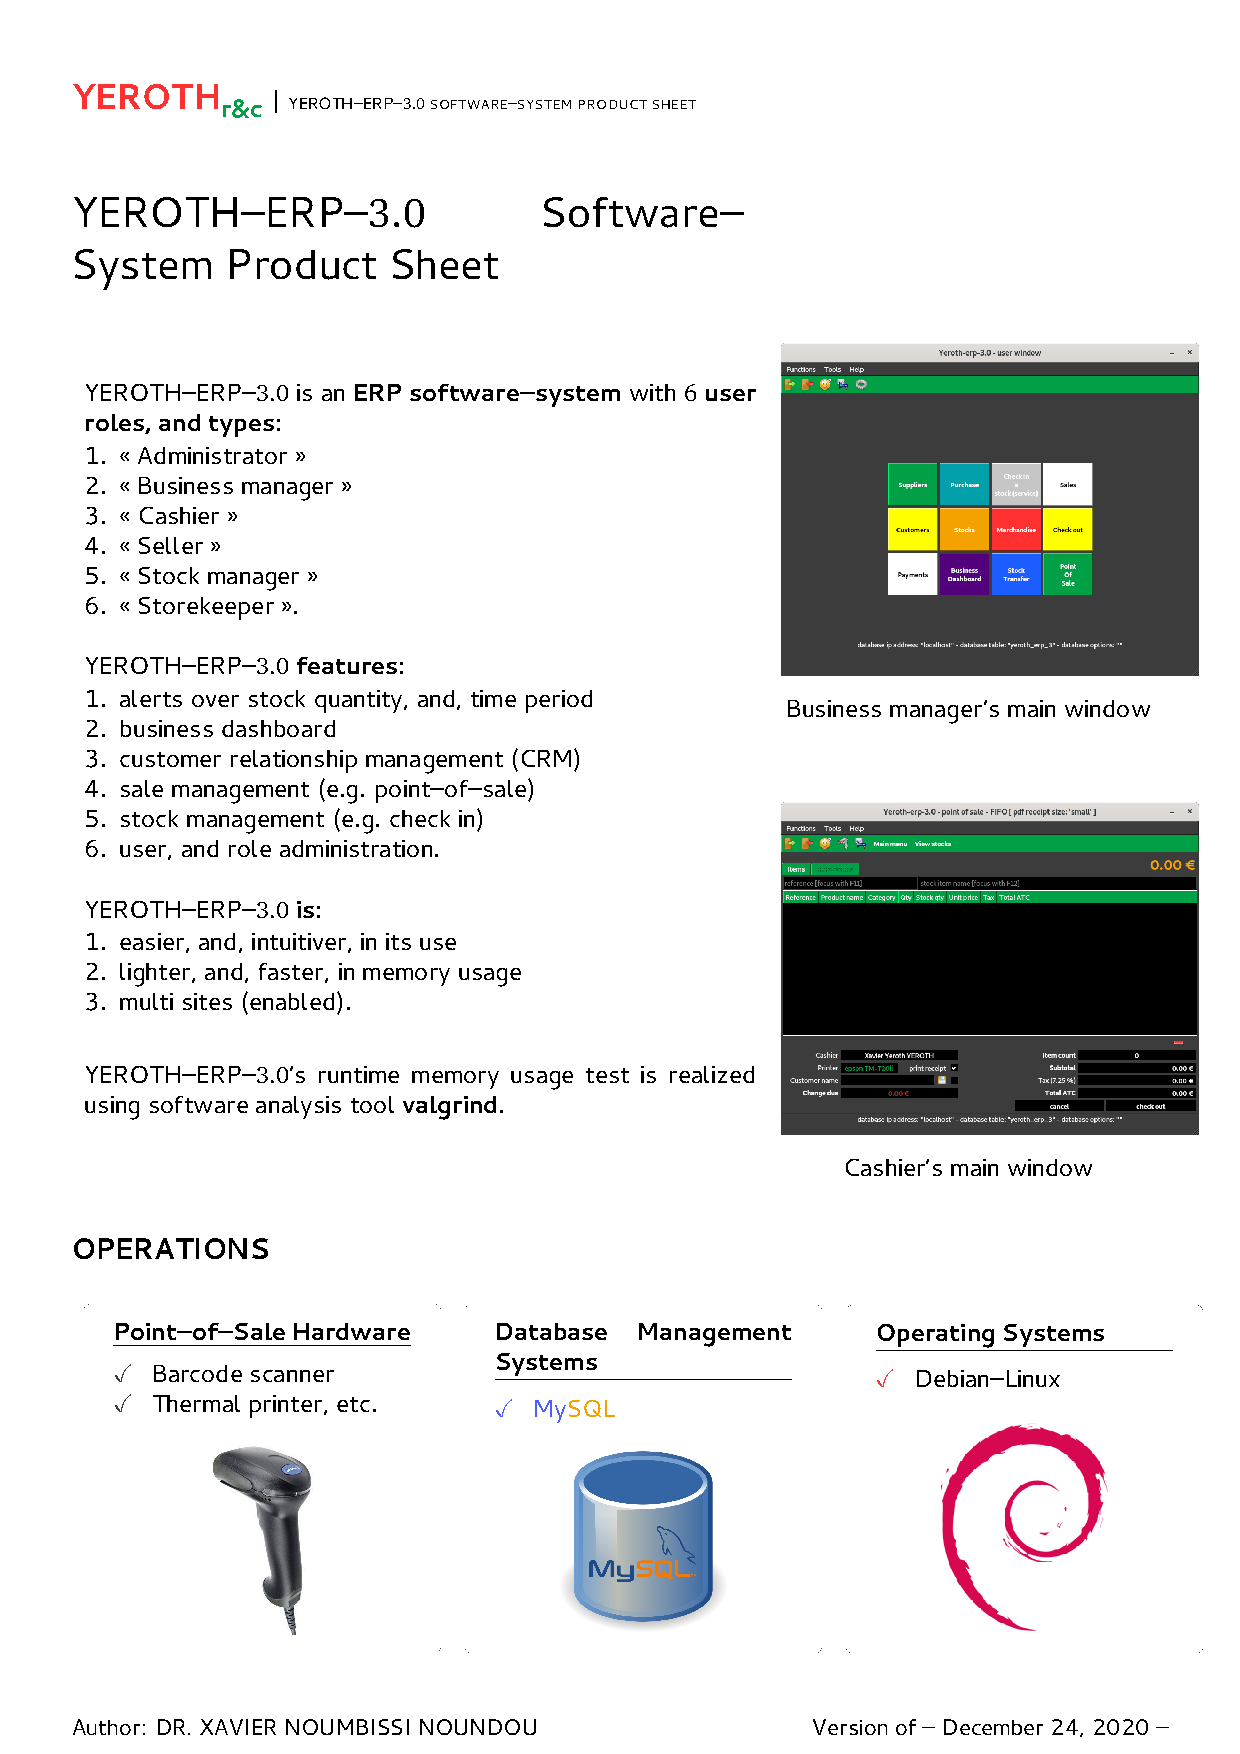
\includegraphics[scale=0.9]{../yeroth-erp-3-0-info-english.pdf}

\newpage
